\documentclass[tikz]{standalone}

\begin{document}

\bfseries
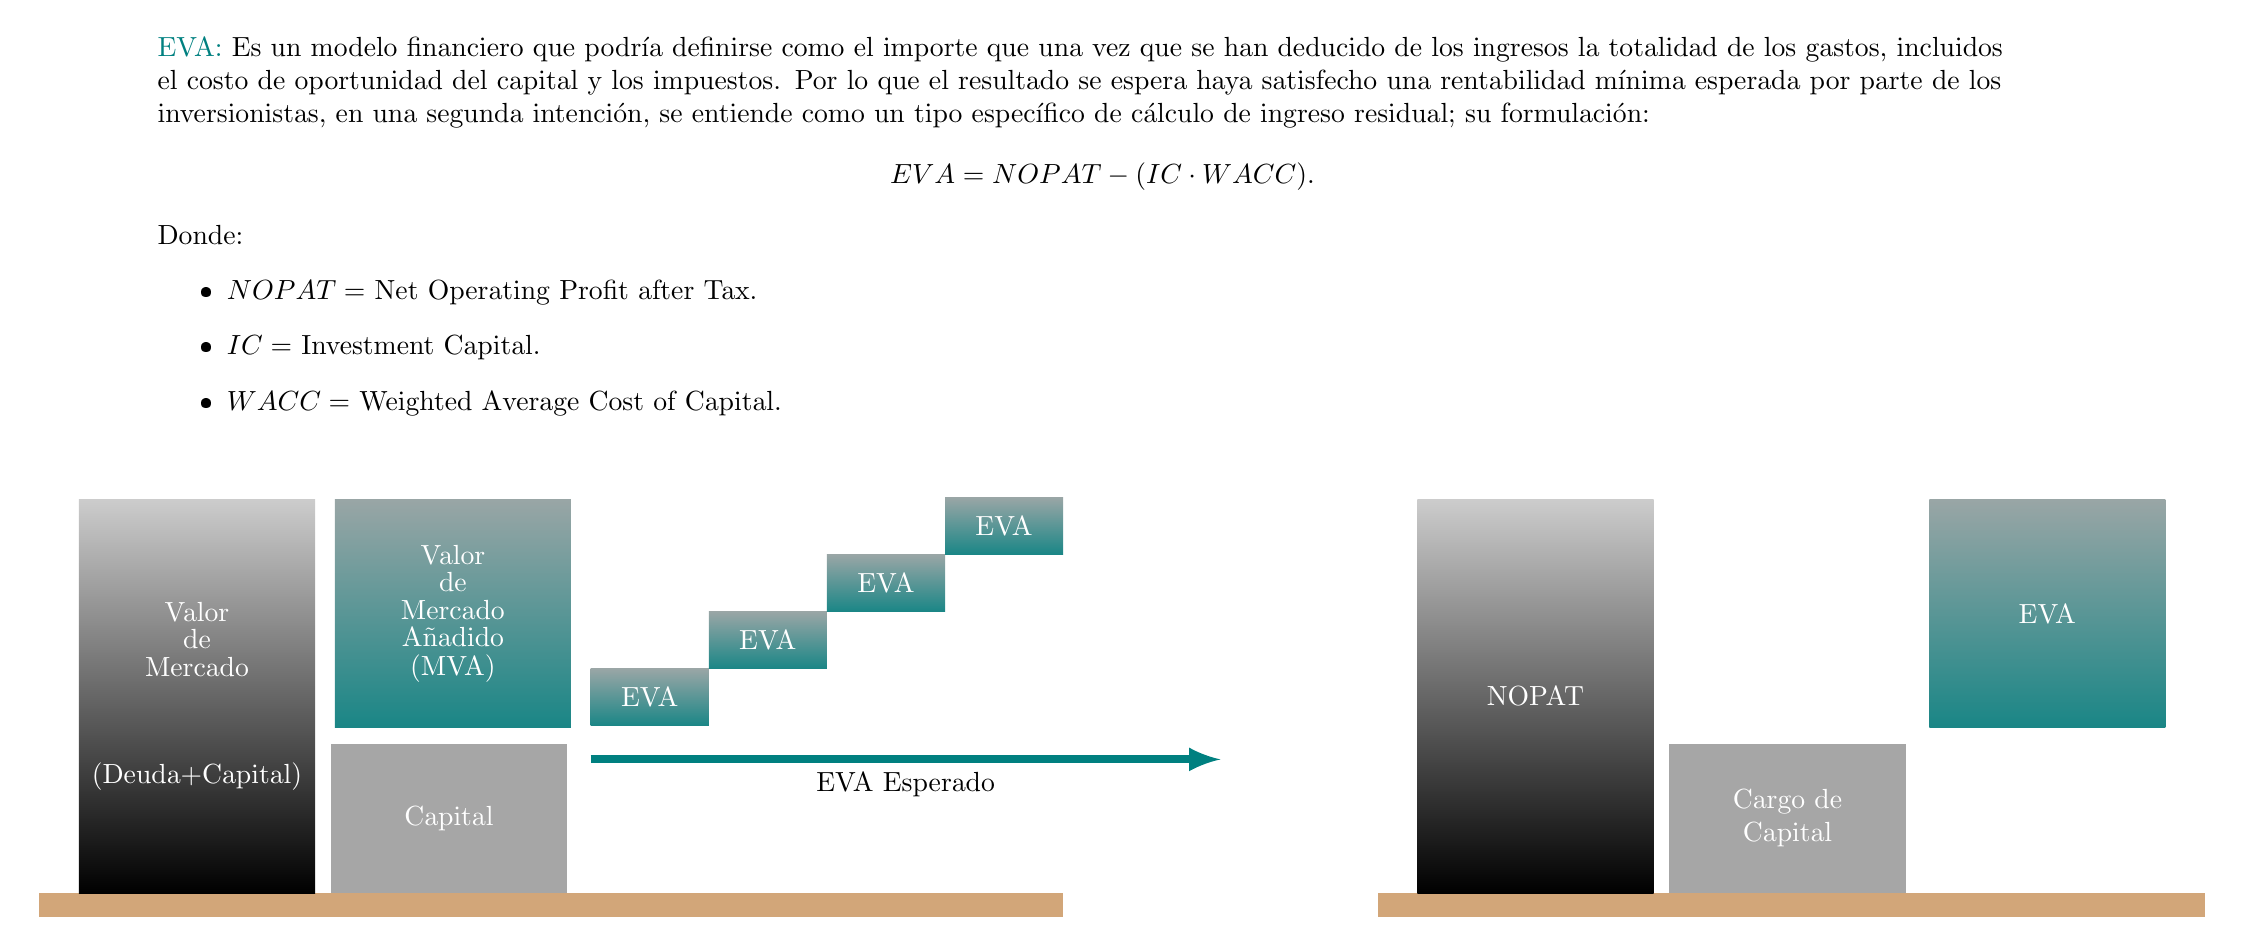
\begin{tikzpicture}
	\node [align=left,anchor=north,text width=24cm] at (10,11) {
		{\color{teal} EVA:} 
		Es un modelo financiero que podría definirse como el
		importe que una vez que se han deducido de los ingresos la totalidad de los
		gastos, incluidos el costo de oportunidad del capital y los impuestos.
		Por lo que el resultado se espera haya satisfecho una rentabilidad mínima
		esperada por parte de los inversionistas, en una segunda intención, se
		entiende como un tipo específico de cálculo de ingreso residual;
		su formulación:
		% Es un modelo financiero que considera la deducción de los gastos 
		\[
			EVA = NOPAT - (IC \cdot WACC).
		\]
		Donde:
		\begin{itemize}
			\item \(NOPAT=\) Net Operating Profit after Tax.
			\item \(IC=\) Investment Capital.
			\item \(WACC=\) Weighted Average Cost of Capital.
		\end{itemize}
	};
	\begin{scope}[xshift=-3cm]
		\draw [line width=3mm, brown!70] (-0.5,-0.15) --++ (13,0);
		\shade [bottom color=black, top color=gray!40] 
		(0,0) rectangle node [text=white] 
		{\shortstack{Valor\\de\\Mercado\\[1cm](Deuda\(+\)Capital)}}
		(3,5);
		\fill [gray!70] (3.2,0) rectangle node [text=white] {Capital} ++(3,1.9);
		\begin{scope}[bottom color=pink!10!teal, top color=pink!60!teal]
		\shade (3.25,2.1) rectangle node [text=white] 
		{\shortstack{Valor \\ de \\ Mercado \\ Añadido \\ (MVA)}} ++(3,2.9);
		\foreach \n in {1,...,4} 
		\shade (6+1.5*\n-1.5+0.5,1.4+\n*0.725) rectangle node [text=white] {EVA} ++(1.5,0.725);
		\end{scope}
		\draw [teal,-latex, line width=1mm] 
		(6.5,1.7) to node[below] {\color{black} EVA Esperado} ++(8,0);
	\end{scope}
	\begin{scope}[xshift=14cm]
		\draw [line width=3mm, brown!70] (-0.5,-0.15) --++ (10.5,0);
		\shade [bottom color=black, top color=gray!40] 
		(0,0) rectangle node [text=white] {\shortstack{NOPAT}} (3,5);
		\fill [gray!70] (3.2,0) rectangle node [text=white] 
		{\shortstack{Cargo de \\ Capital}} ++(3,1.9);
		\shade [bottom color=pink!10!teal, top color=pink!60!teal] 
		(6.5,2.1) rectangle node [text=white] {EVA} ++(3,2.9);
	\end{scope}
\end{tikzpicture}

\end{document}
